\documentclass{beamer}
\title{Intersemsterial Presentation}
\author{Arthur Adriaens}
\date{\today}
\usetheme{Boadilla}
\useoutertheme{infolines}

\begin{document}
\begin{frame}
	\titlepage
\end{frame}
\begin{frame}{Setup}
  \begin{itemize}
    \item The need for RNO-G
    \item RNO-G
    \item Ice Models
    \item My work
  \end{itemize}
\end{frame}
\begin{frame}{The need for RNO-G}
  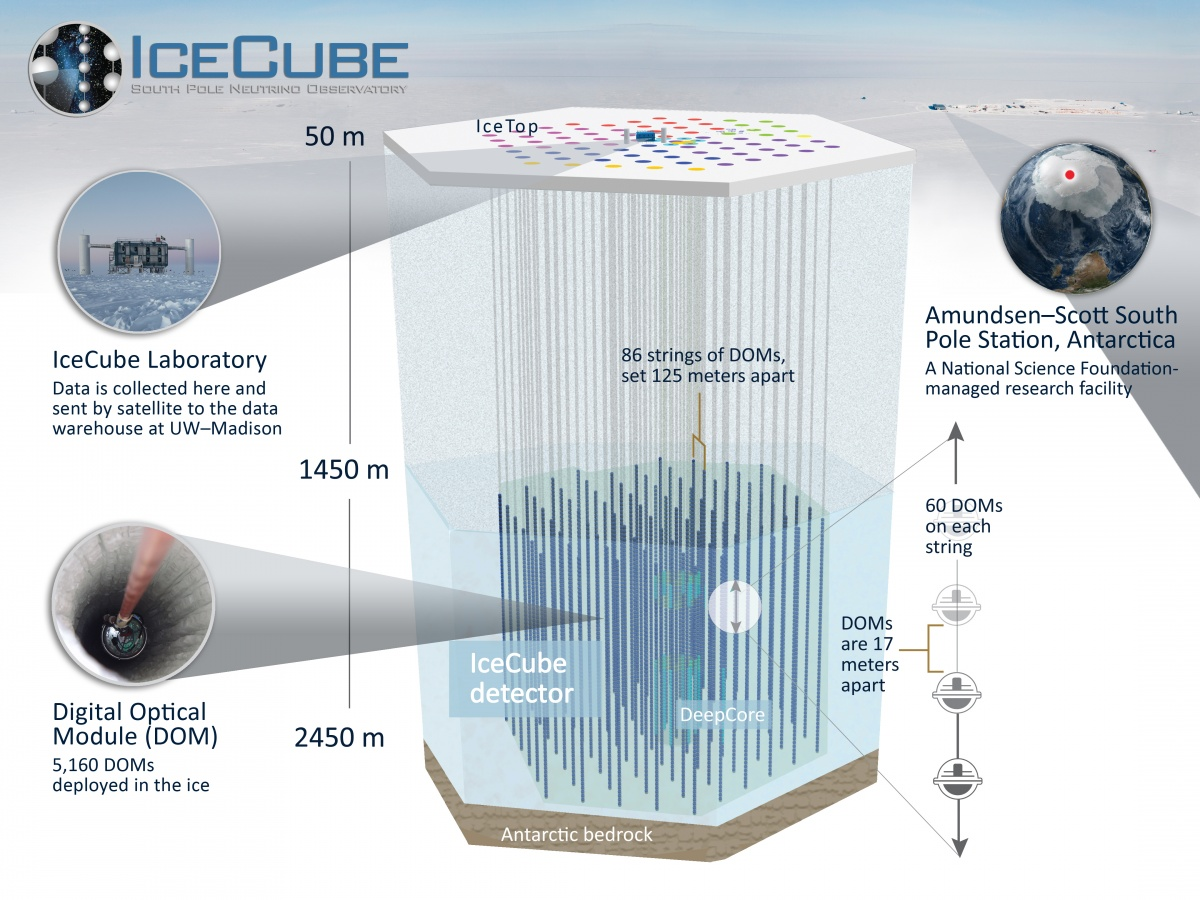
\includegraphics[height=0.9\textheight]{figures/icecube.jpg}
\end{frame}
\begin{frame}{The need for RNO-G}
  IceCube finds no events for energies $> 3PeV$ (\it{IceCube study of down-going neutrinos for the spectral cutoff determination by 
Palczewski and Tomasz})
\end{frame}
\begin{frame}{The need for RNO-G}
  \centering
  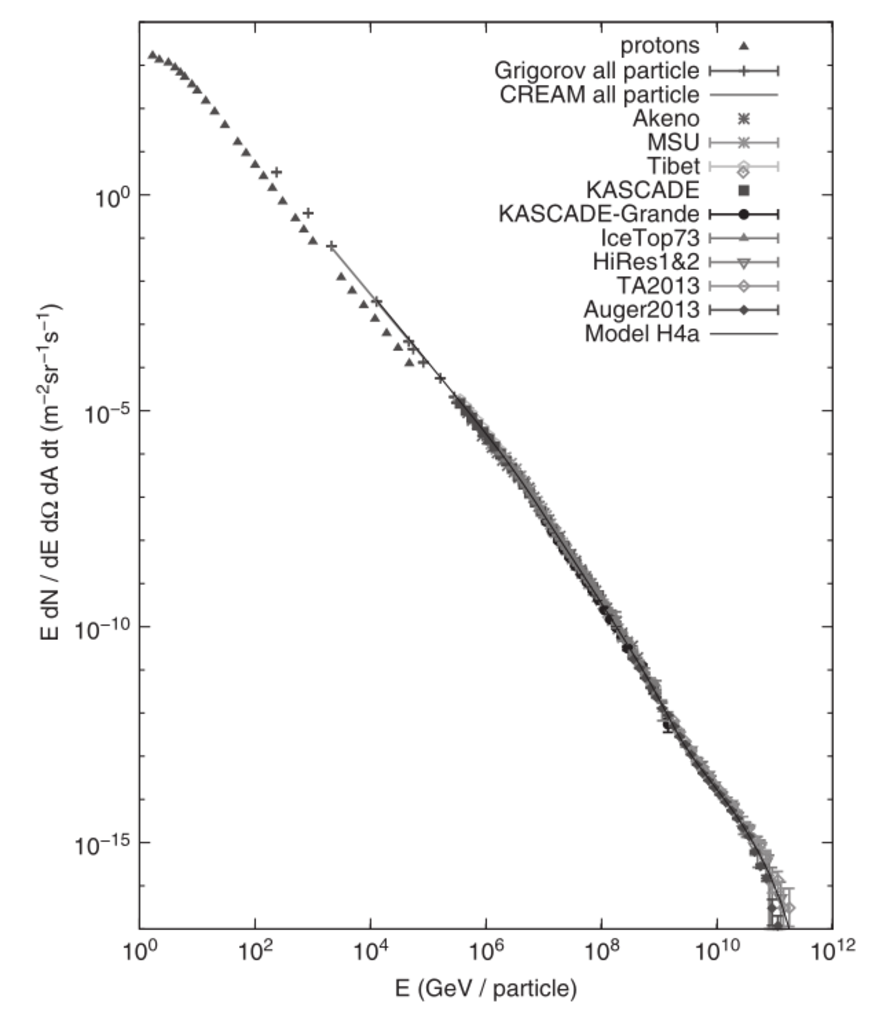
\includegraphics[height=0.9\textheight]{figures/cosmic_ray_flux.pdf}
\end{frame}
\begin{frame}{RNO-G}
  Problem: visible light doesn't travel far in ice\\
  $\rightarrow$ Solution: radio waves
\end{frame}
\begin{frame}{RNO-G}
  \centering
  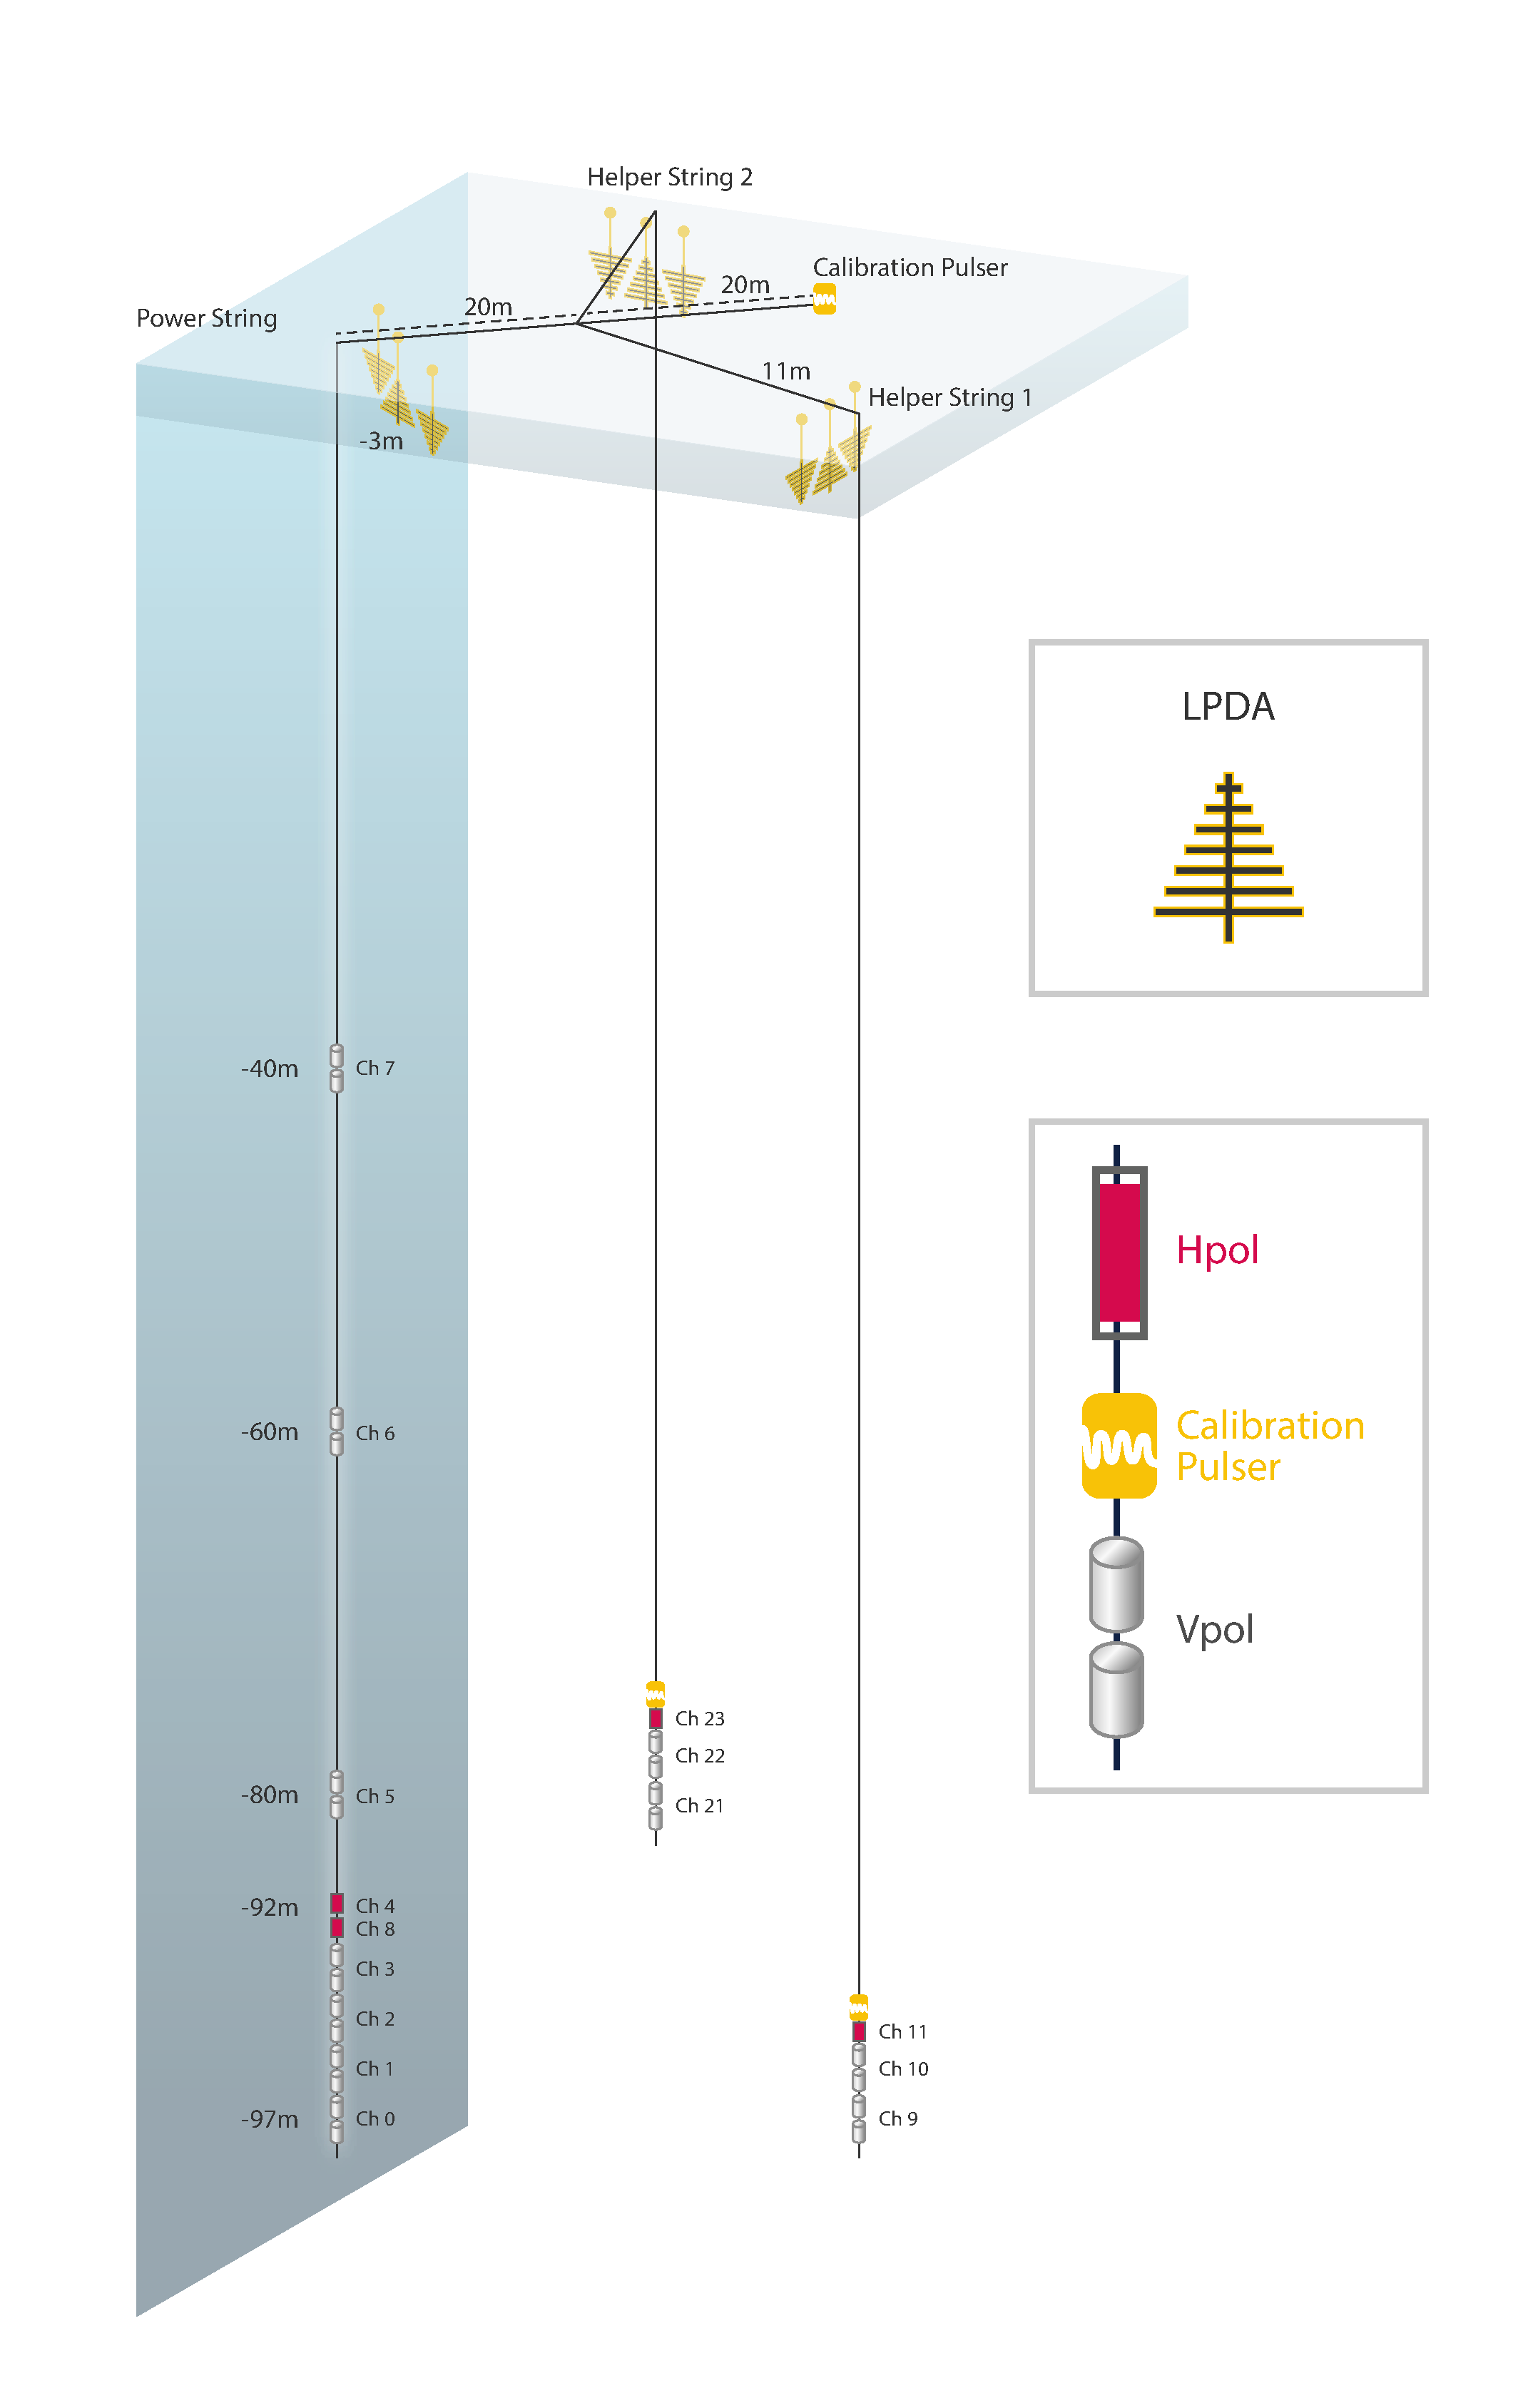
\includegraphics[height=0.9\textheight]{figures/detector.pdf}
\end{frame}
\begin{frame}{RNO-G}
  \centering
  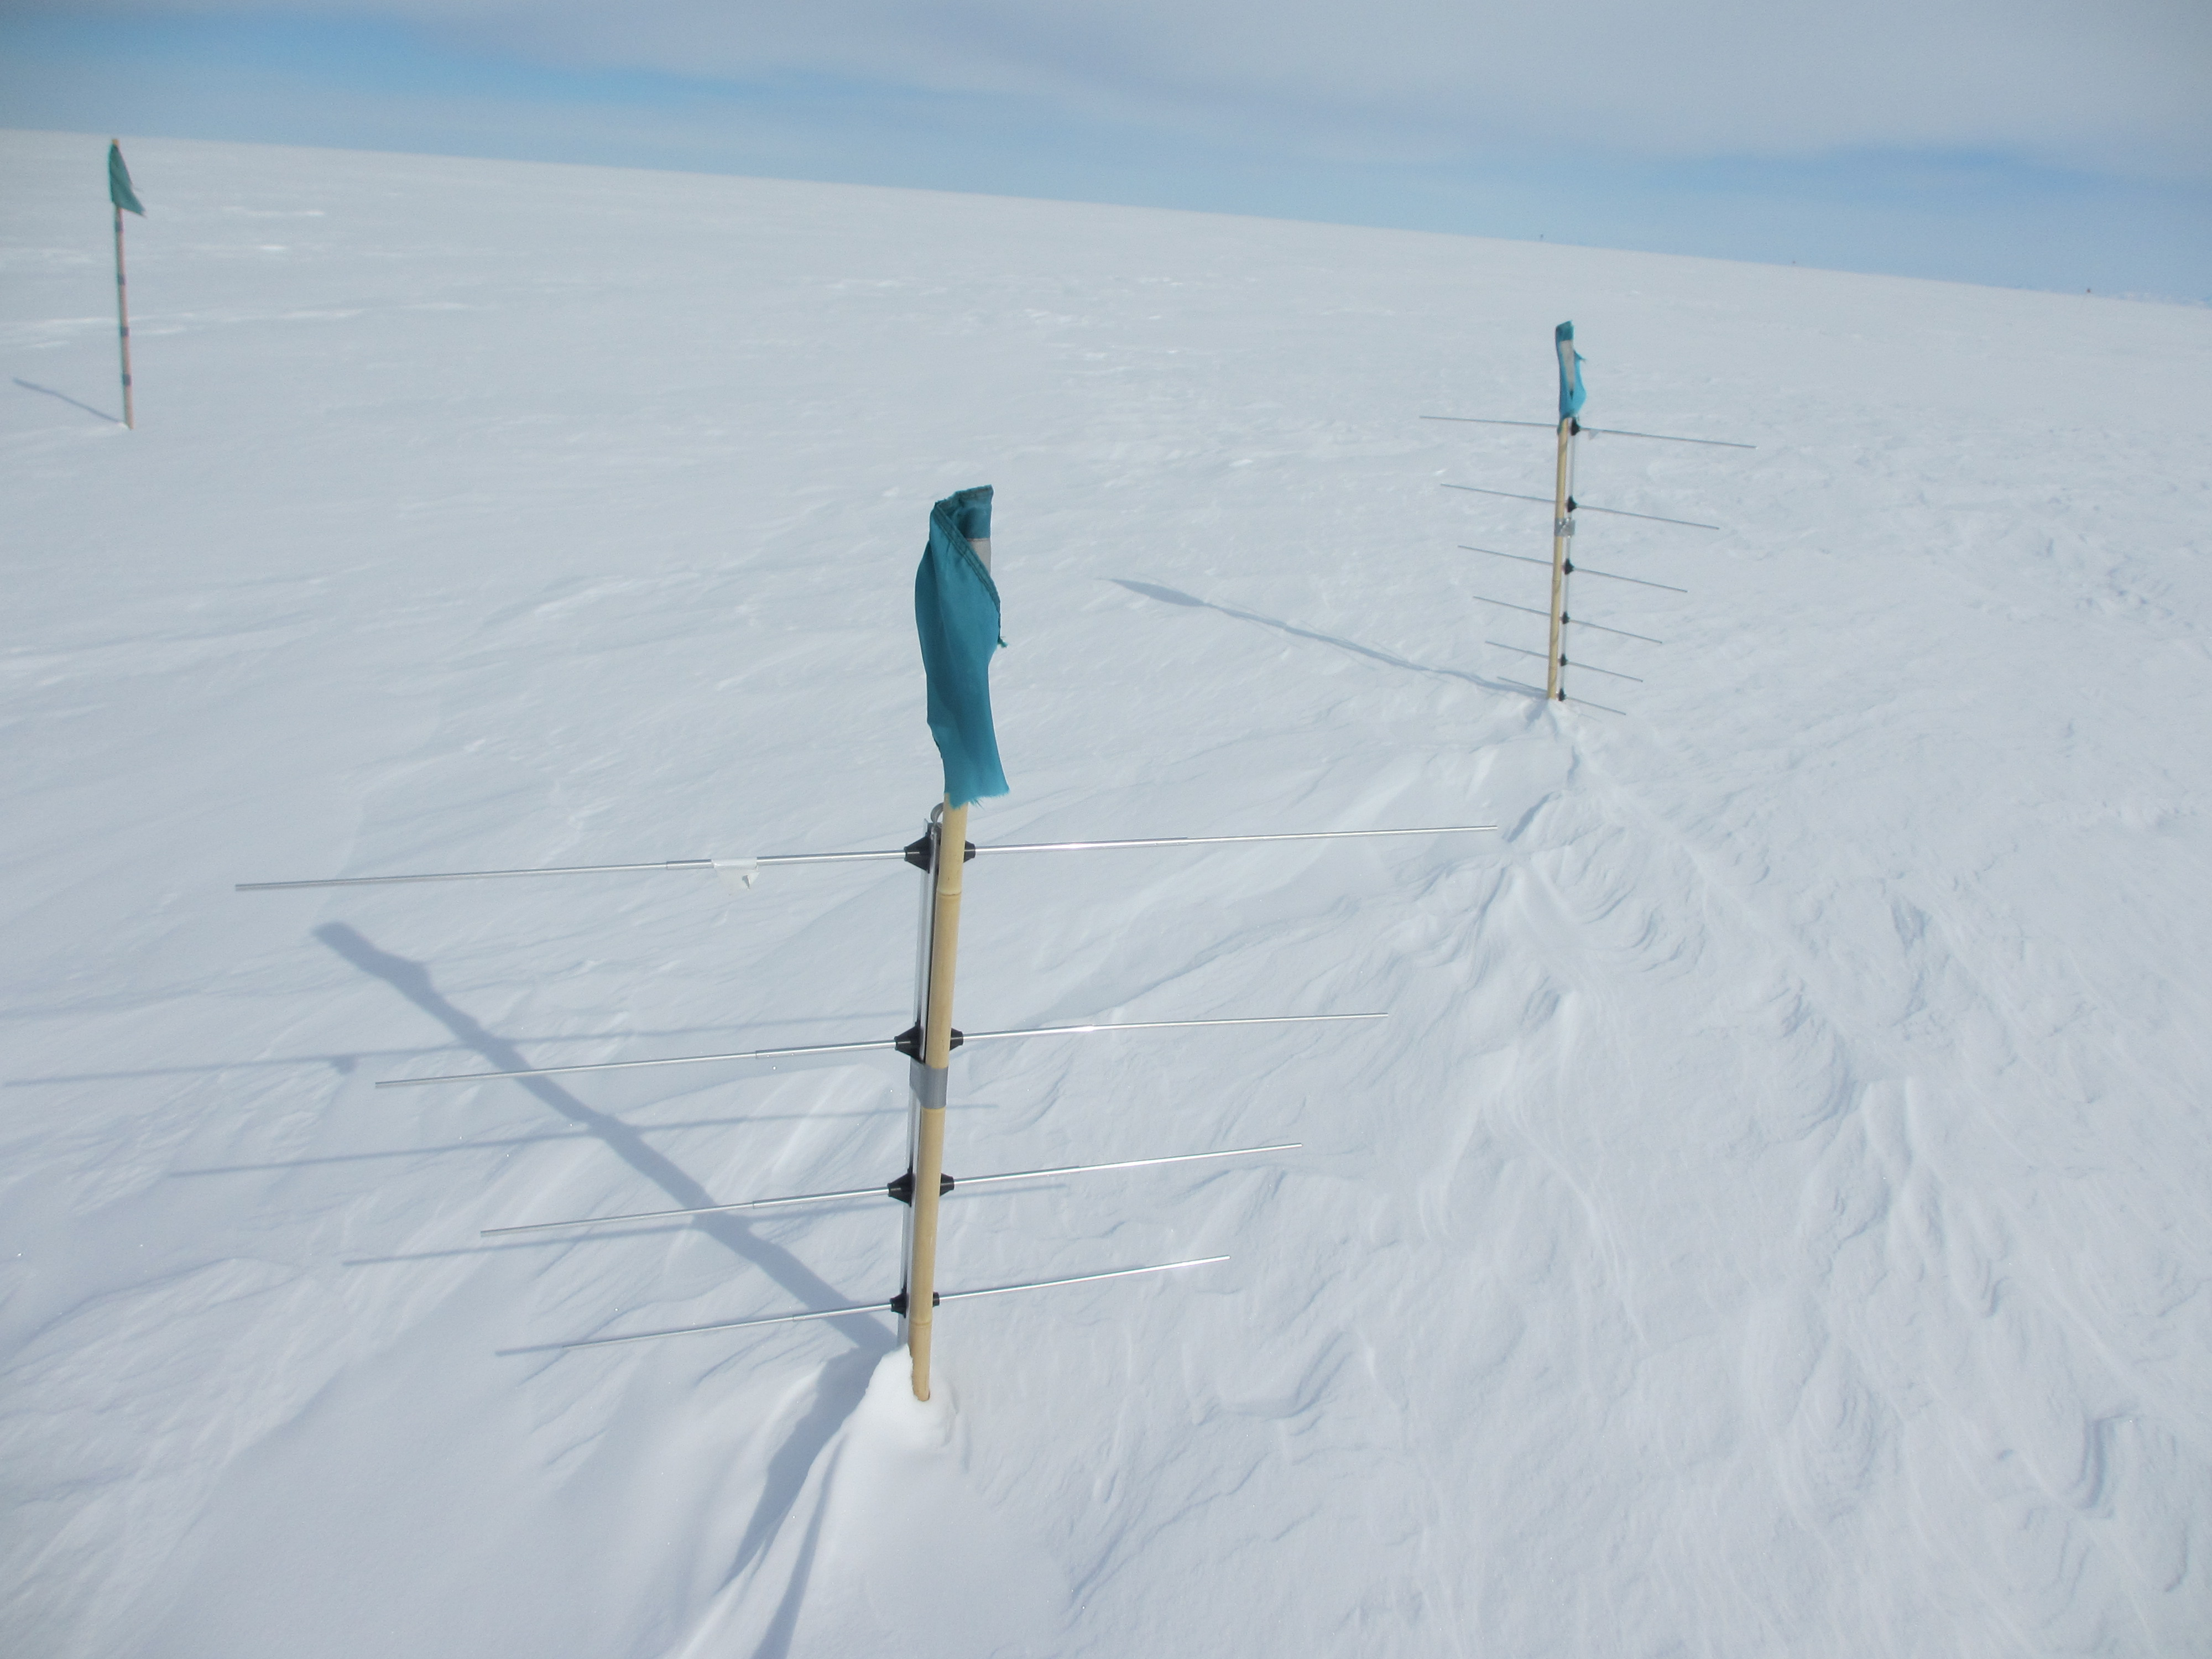
\includegraphics[height=0.8\textheight]{figures/highlight.jpg}
\end{frame}
\begin{frame}{RNO-G}
  \centering
  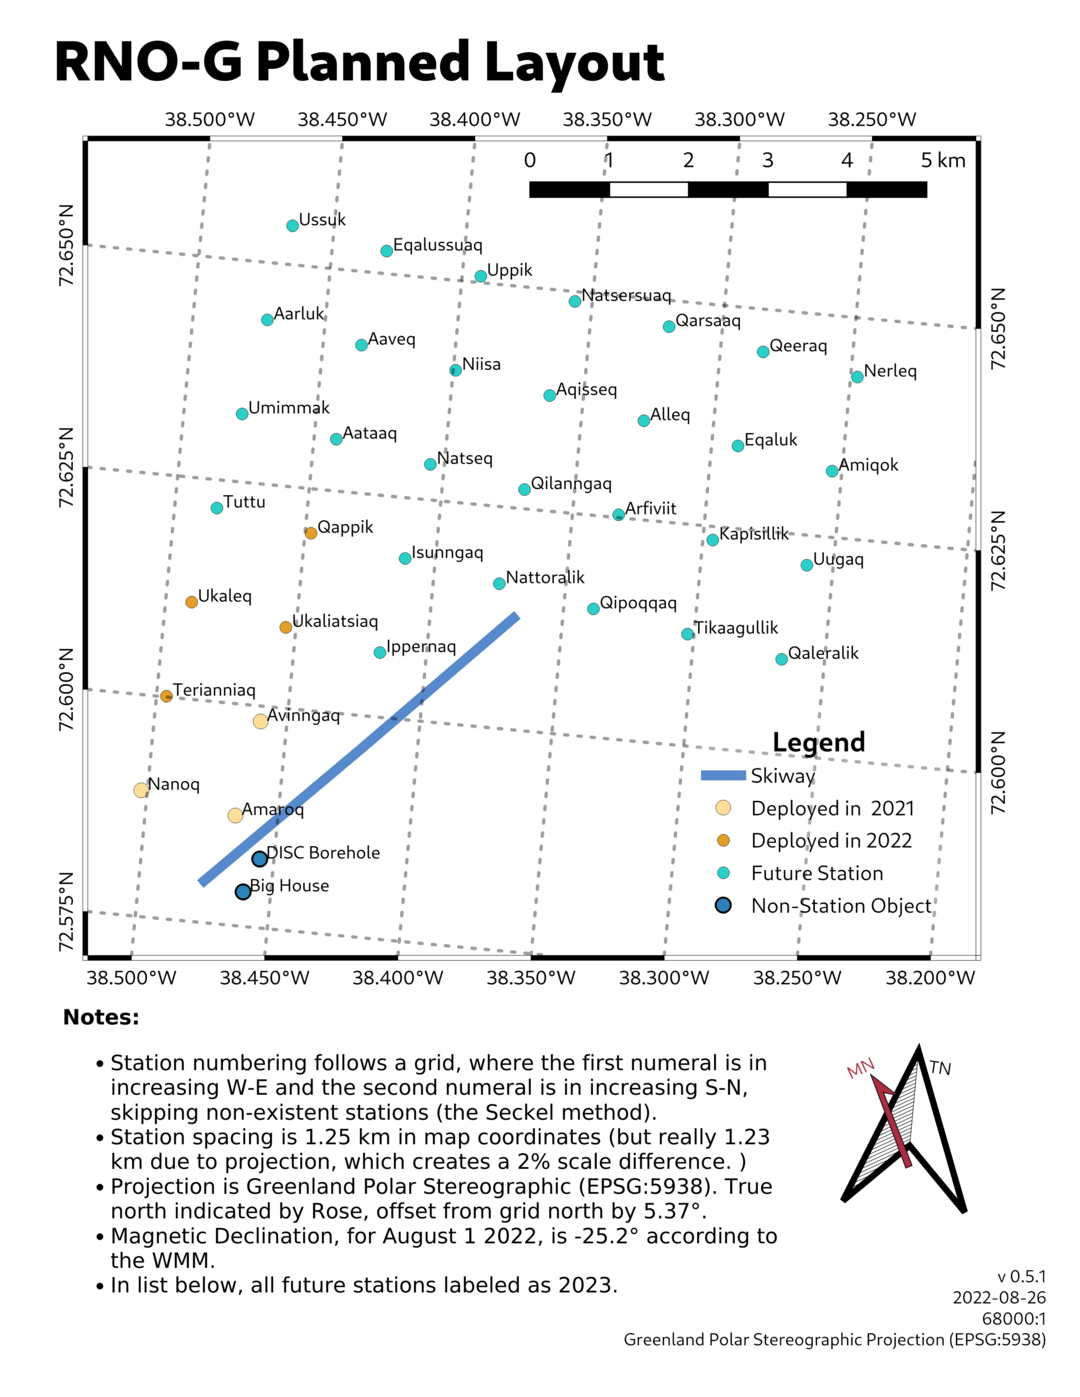
\includegraphics[height=\textheight]{figures/station-map.png}
\end{frame}
\begin{frame}{Ice Models}
  \centering
  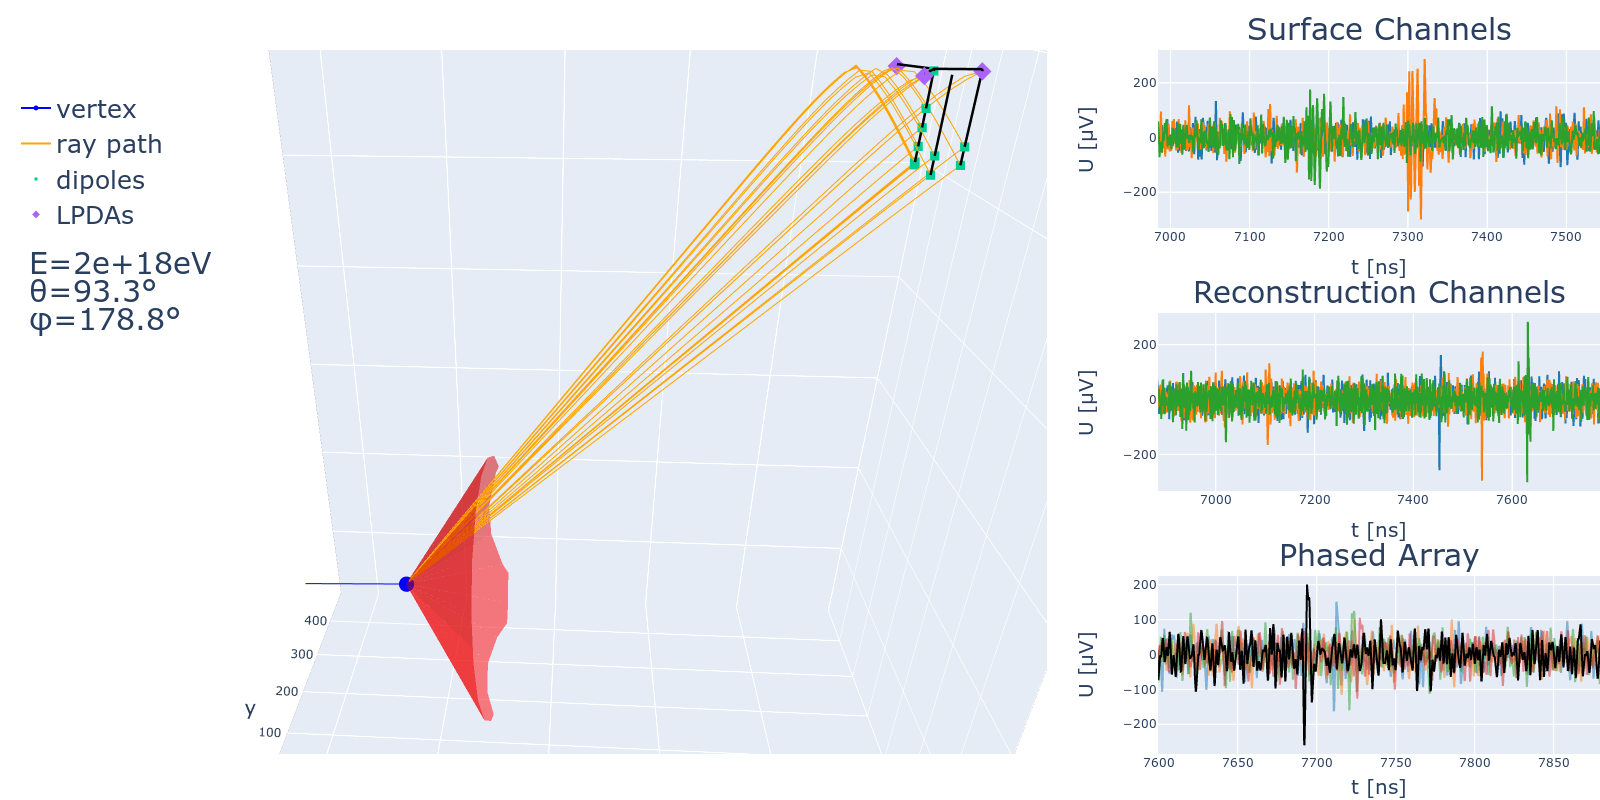
\includegraphics[width=\textwidth]{figures/mechanism.png}
\end{frame}
\begin{frame}{Ice Models}
Eikonal:
  \begin{equation}
    \mathbf{\nabla} n \approx n(\mathbf{r})\frac{d^2\mathbf{r}}{ds^2}
  \end{equation}
Exponential model:
  \begin{equation}
    n(z) = n_0 - \Delta n \ e^{-z/z_0}
  \end{equation}
\end{frame}
\end{document}
